\documentclass{article}
\usepackage{graphicx} % Required for inserting images

% Para los ejercicios
\usepackage{amsmath, amsfonts, amsthm}
\usepackage{thmtools}
\usepackage[utf8]{inputenc} %Para los acentos
\usepackage{mdframed}	%Para los colorsitos en los teoremas


%%Para el cuadrado negro
\usepackage{amssymb}

%%Para el seno
\newcommand{\sen}{\textrm{sen}}

% Estilo general
\declaretheoremstyle[
headfont=\normalfont\bfseries,
bodyfont=\normalfont
]{normal}

% Para problemas
\declaretheorem[style = normal, name = Problema]{problema}

% Para teoremas
\declaretheorem[style = normal, name = Teorema]{teorema}

% Para lemas
\declaretheorem[style = normal, name = Lema, numbered = no]{lema}

% Para ejercicios
\declaretheorem[style = normal, name = Ejercicio]{ejercicio}

% Para ejemplos
\declaretheorem[style = normal, name = Ejemplo]{ejemplo}

% Para observaciones
\declaretheorem[style = normal, name = Observación, numbered = no]{observacion}

% Para demostraciones y soluciones
\declaretheoremstyle[%
	headpunct={\\[3pt]}
]{solstyle}

% Para demostraciones
\declaretheorem[style = solstyle, name = Demostración, numbered = no]{demostracion}

% Para soluciones
\declaretheorem[style = solstyle, name = Solución, numbered = no]{solucion}


\title{Algunas formas de trabajar con tangente}
\author{Neftalí Adolfo Maceda Espinosa}

\begin{document}

\maketitle

% Lema previo para el criterio de la tangente
\section*{Tangentes a circunferencias.}

Probablemente ya has escuchado el término "recta tangente a una 
circunferencia". Si te mostrarán una imagen de una circunferencia y un recta,
probablemente podrías decir si dicha recta es tangente a la circunferencia.
Sin embargo, cuando se trata de problemas de geometría donde están involucradas
una o más rectas tangentes a una circunferencia, lo más seguro es que la idea
intuitiva de qué es una tangente no te lleve a resolver el problema. Más aún,
si te piden demostrar que una recta es tangente a una circunferencia, tal vez
no tengas muchas herramientas para hacerlo. Por tal motivo, en este artículo
te mostraré algunas formas de trabajar con problemas que involucren rectas
tangentes a circunferencias, y también una que otra circunferencia tangente
a otra circunferencia.\\

Primero que nada, ¿qué es una recta tangente a una circunferencia? Bueno, si 
tenemos una recta $l$ y una circunferencia $\Omega$, entonces se dice que la
recta $l$ es tangente a $\Omega$ si $l$ corta a $\Omega$ en un único punto. 
Esto quiere decir dos cosas: La recta $l$ sí corta a $\Omega$, y además
ese punto debe ser único, no puede haber otro punto de intersección entre 
$l$ y $\Omega$. Esto suena interesante. Sin embargo, a la hora de trabajar
con problemas reales de concurso, el hecho de que haya un único punto de 
intersección entre una circunferencia y una recta no te da mucha información.\\

Uno de los primeros resultados sobre tangentes relaciona la recta en cuestión 
con uno de los elementos más importantes sobre circunferencias: su centro.
El siguiente resultado te ayuda no solo a obtener más datos a partir de una
tangencia. También te ayuda en caso de que quieras probar que una recta es
tangente a una circunferencia en un punto dado.

\newpage
\begin{lema}
    Sea $\Omega$ una circunferencia con centro $O$, y sea $P$ un punto
    sobre la misma. Además, sea $l$ una recta que pasa por $P$. Se tiene
    que $l$ es tangente a $\Omega$ en $P$ si y sólo si $l$ es perpendicular
    a $OP$.
\end{lema}


\begin{demostracion}
    Comencemos por demostrar que si $OP$ es perpendicular a la recta $l$,
    entonces $l$ es tangente a $\Omega$. Para ello, haremos algo que no es muy
    común en geometría de olimpiada: usar contradicción. Supongamos que $l$ no es tangente
    a $\Omega$ en $P$. Nosotros ya sabemos que $l$ intersecta a $\Omega$ en 
    el punto $P$. Por tal razón, si $l$ no es tangente a $\Omega$ en $P$,
    entonces debe existir otro punto $Q$ distinto de $P$ que está en $l$
    y en $\Omega$.\\

    Aquí es donde se pone un poco truculenta la cosa. Para llegar a una 
    contradicción, consideraremos el punto medio de $PQ$. Denotemos por $M$
    a dicho punto. Como $P$ y $Q$ son puntos de la circunferencia,
    $OP = OQ$, lo cual implica que el triángulo $\triangle OPQ$ es isósceles.
    Luego, al ser $M$ el punto medio de $PQ$, debe cumplirse que 
    $OM$ es perpendicular a $PQ$, y por tanto que $OM$ es perpendicular a $l$.
    No obstante, nosotros sabemos que $OP$ es perpendicular a $l$. En 
    consecuencia, debe cumplirse que $P=M$, contradiciendo el hecho de que
    $M$ es el punto medio de $PQ$. Así, concluimos que $l$ es tangente a 
    $\Omega$ en $P$.

    \begin{figure}[h]
        \centering
        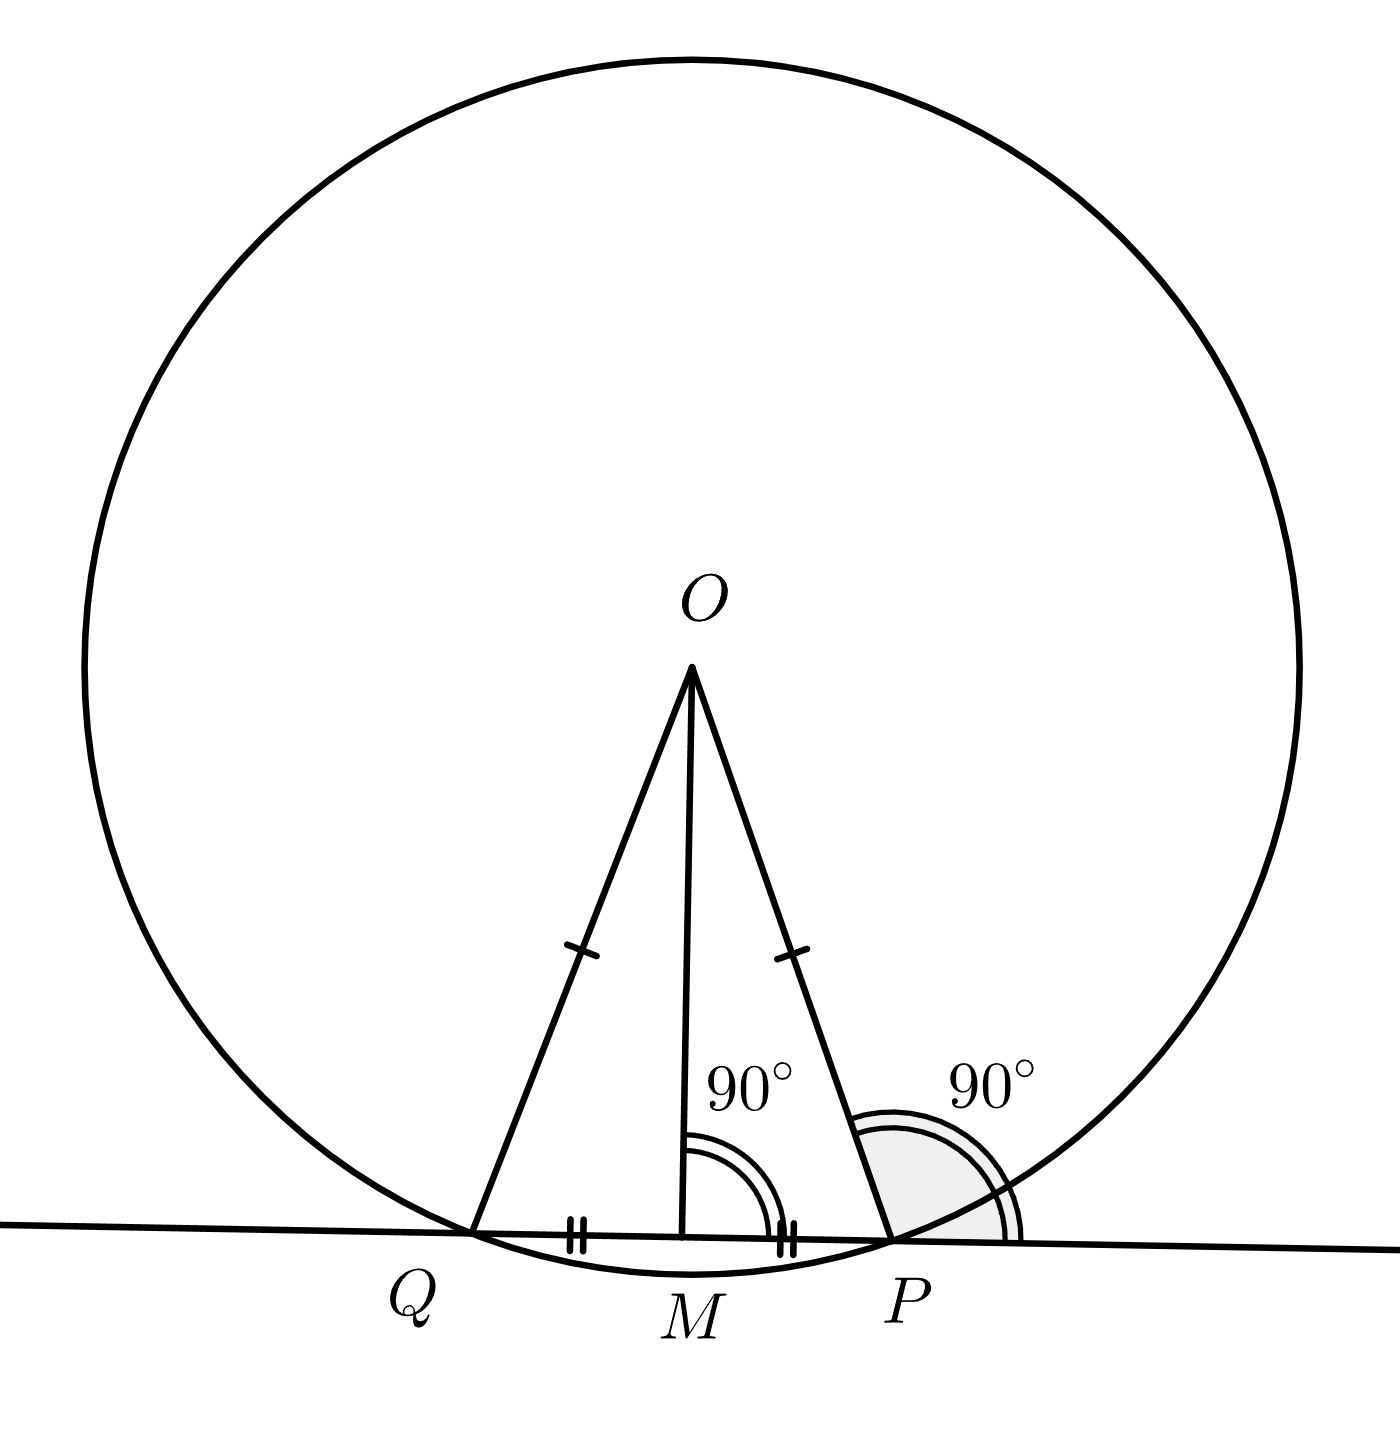
\includegraphics[width=0.7\linewidth]{images/t1i1.png}
    \end{figure}

    Supongamos ahora que $l$ es tangente a $\Omega$ en $P$. En esta ocasión,
    queremos demostrar que $OP$ es perpendicular a $l$.\\

    \newpage
    Tal vez ya hayas adivinado lo que vamos a hacer en este caso. Nuevamente,
    vamos a usar contradicción. Supongamos que $OP$ no es perpendicular a $l$,
    y sea $M$ el pie de la perpendicular desde $O$ hacia la recta $l$. 
    Como $OP$ no es perpendicular a $l$, entonces debería cumplirse que 
    $P \neq M$, razón por la cual es posible tomar la reflexión de $P$
    con respecto a $M$, digamos $Q$. Por definición de reflexión, $Q$ es 
    un punto sobre $l$ que satisface que $M$ es el punto medio de $PQ$.
    Además, ya que $OM$ es perpendicular a $l$, entonces también $OM$ es
    perpendicular a $PQ$. Luego, $O$ está sobre la mediatriz de $PQ$, de
    lo cual se sigue que $OP = OQ$. Sin embargo, nosotros sabemos que $OP$
    es un radio de $\Omega$. Por lo tanto, $OQ$ también debe ser un radio de
    $\Omega$, lo cual implica que $Q$ también está en $\Omega$, pero esto
    contradice el supuesto de que $l$ es tangente a $\Omega$ en $P$. En 
    consecuencia, concluimos que $OP$ es perpendicular a $l$. $\blacksquare$

    \begin{figure}[h]
        \centering
        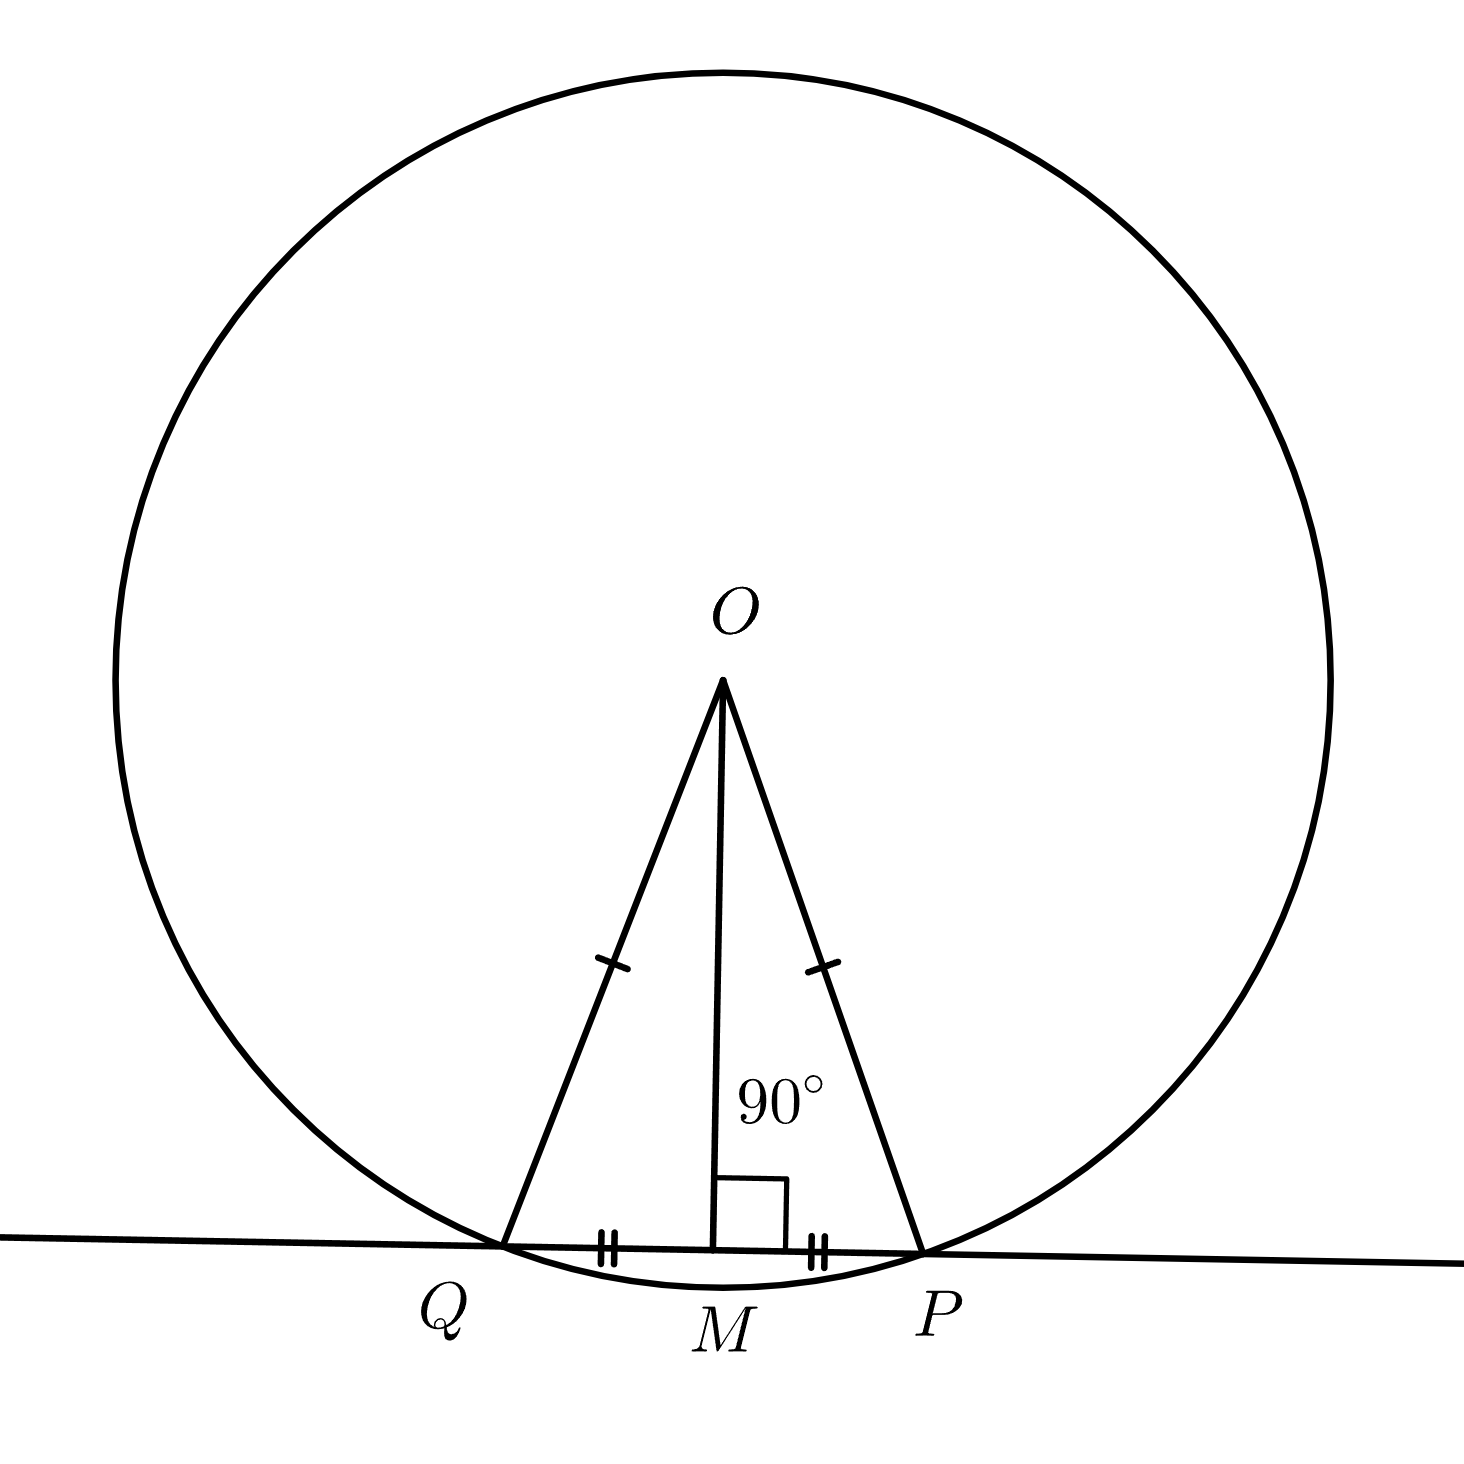
\includegraphics[width=0.7\linewidth]{images/t1i2.png}
    \end{figure}
\end{demostracion}

El lema que acabamos de demostrar ya nos da un poquito más de información. Por
lo menos sabemos que si tenemos el centro y una tangente, entonces ahí debe
haber perpendicularidad, y esto nos puede ayudar a probar cíclicos, congruencias,
semejanzas, entre muchas otras cosas. Sin embargo, cuando no se tiene
directamente el centro de la circunferencia sino, por ejemplo, tres puntos
por los que pasa, el lema previo ya no es tan útil de forma directa. Es por 
tal razón que el siguiente teorema, a veces conocido como el Criterio 
de la tangente, suele ser de los más poderosos a la hora de lidiar con tangentes.

\newpage

\begin{teorema}[\textbf{Criterio de la tangente}]
    Sea $\triangle ABC$ un triángulo con circuncírculo $\Omega$ y 
    circuncentro $O$, y sea $P$ un punto distinto de $B$ y de $C$ tal que
    $A$ y $P$ están en lados opuestos de $BC$. Son equivalentes:\\

    \begin{enumerate}
        \item $PC$ es tangente a $\Omega$ en $C$.
        \item  $OC$ es perpendicular a $PC$.
        \item $\angle PCB = \angle CAB$.
    \end{enumerate}
\end{teorema}

\begin{demostracion}
    Por el lema previo, sabemos de antemano que 1 y 2 son equivalentes, por
    lo cual solo tenemos que demostrar que 2 y 3 son equivalentes. Para ello,
    comencemos por hacer algunas observaciones. En primera, denotemos por 
    $\angle PCB = \alpha$. Notemos que al ser $B$ y $C$ puntos sobre $\Omega$,
    el triángulo $triangle OBC$ es isósceles con $OB = OC$, lo cual implica
    que $\angle BCO = \angle OBC$. Además, por el teorema del ángulo inscrito,
    $\angle COB = 2\angle CAB$. Sabiendo esto, demostremos primero 
    que si 2. se cumple, entonces 3. también.\\

    Supongamos que $OC$ es perpendicular a $PC$. Es claro entonces que 
    $\angle BCO = 90^{\circ} - \angle PCB = 90 - \alpha$. Luego, ya que
    el $\triangle OBC$ es isósceles con $OB = OC$, de lo anterior se sigue
    que $\angle COB = 2\alpha$. Así, ya que $\angle COB = 2\angle CAB$,
    se sigue que $\angle CAB = \alpha$, por lo cual concluimos que
    $\angle PCB = \angle CAB = \alpha$.\\

    Supongamos ahora que $\angle CAB = \angle PCB = \alpha$. Entonces debe
    cumplirse que $\angle COB = 2\angle CAB = 2\alpha$. Usando ahora
    el hecho de que el triángulo $\triangle OBC$ es isósceles, se deduce
    que $\angle BCO = 90^{\circ} - \alpha$. Así,
    $\angle PCO = \angle PCB + \angle BCO = 90^{\circ}$, probando que
    $OC$ es perpendicular a $PC$. Por tanto, concluimos que 2. y 3. son
    equivalentes. $\blacksquare$

    \begin{figure}[h]
        \centering
        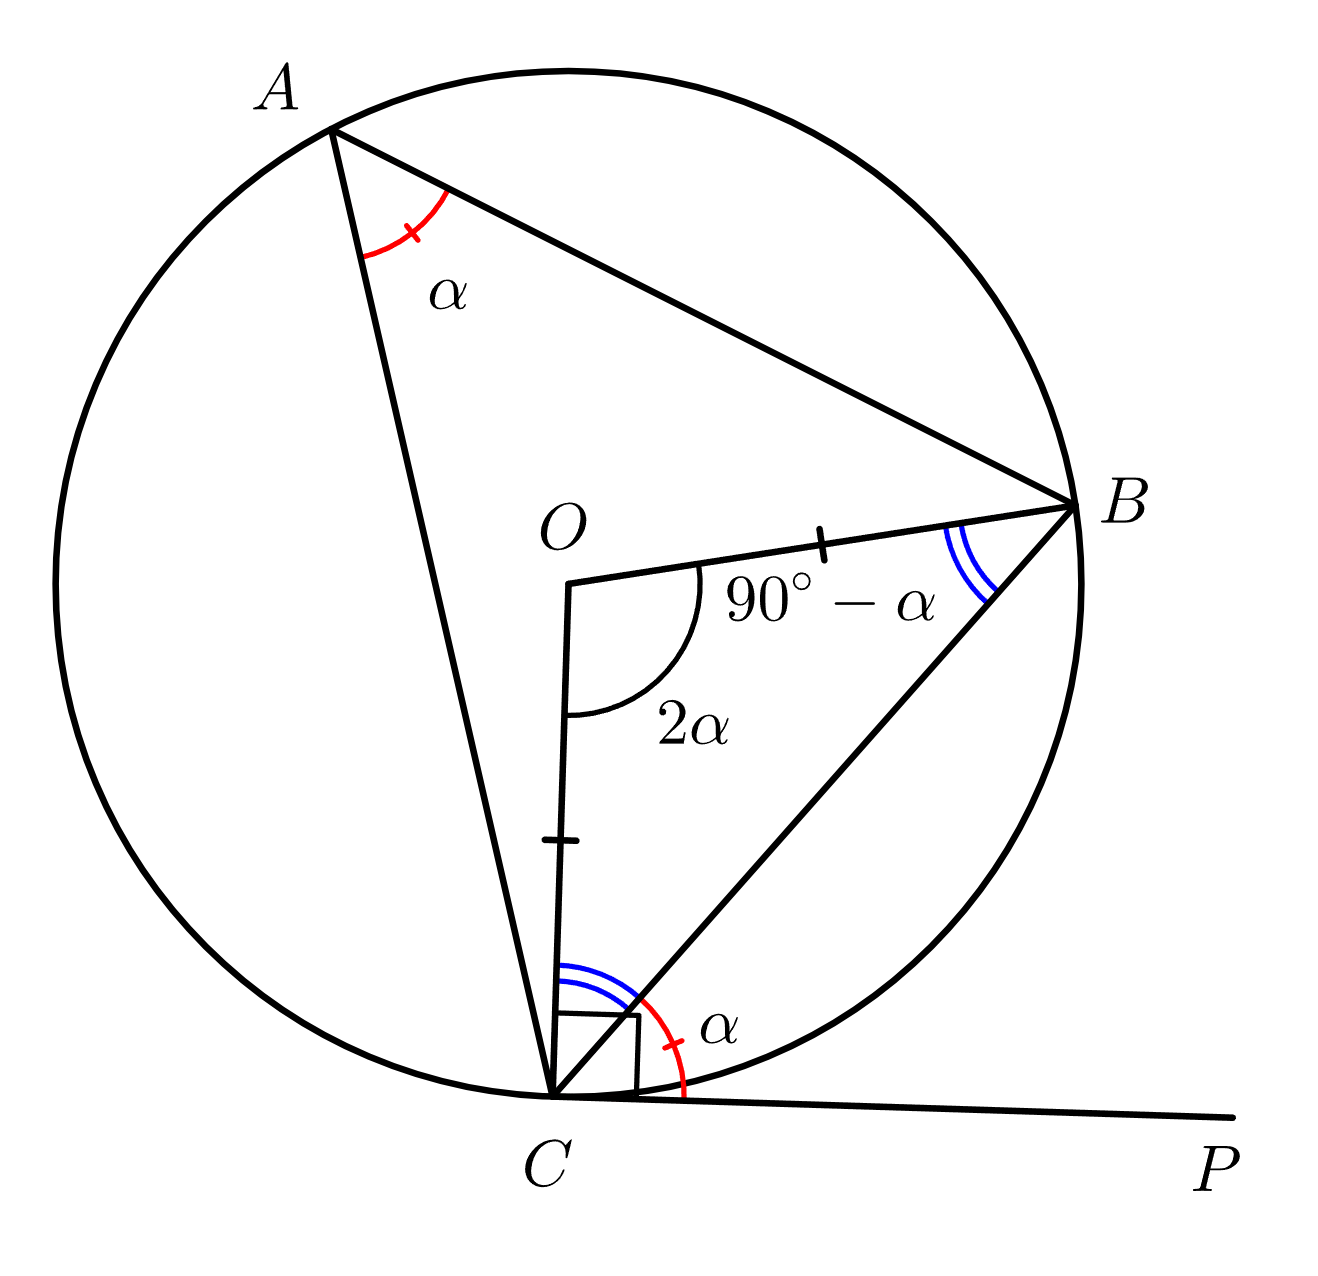
\includegraphics[width=0.55\linewidth]{images/t2i1.png}
    \end{figure}
\end{demostracion}

Ahora sí ya tenemos una herramienta sumamente útil para encargarnos de los
problemas de tangentes, al menos siempre y cuando necesitemos cosas relacionadas
con ángulos. Un caso particular del teorema anterior es cuando el triángulo
$\triangle ABC$ es isósceles. En este caso, es posible que para probar que
$l$ es tangente al circuncírculo solo haya que demostrar que $l$ es tangente
a alguno de los lados. Esto lo veremos en el siguiente teorema:\\

\begin{teorema}
    Sea $\Omega$ una circunferencia y sean $A, B$ y $C$ puntos distintos sobre
    la misma. Además, sea $l$ la recta tangente a $\Omega$ en $A$. 
    Entonces el triángulo $\triangle ABC$ es isósceles con 
    $AB = AC$ si y sólo si $l$ es paralela a $BC$.
\end{teorema}

\begin{demostracion}
    Sea $P$ un punto sobre $l$ tal que $B$ y $P$ están en lados opuestos de la
    recta $AC$. Observamos entonces que, por el Criterio de la tangente,
    $\angle CAP = \angle CBA$. Sabiendo esto, supongamos en primera que
    el triángulo $\triangle ABC$ es isósceles con $AB = AC$. Luego,
    $\angle CBA = \angle ACB$, pero ya que $\angle CAP = \angle CBA$,
    entonces debe cumplirse que $\angle CAP = \angle ACB$, implicando
    que $l$ es paralela a $BC$.\\

    Por otro lado, si $l$ es paralela a $BC$, entonces se tiene que
    $\angle CAP = \angle ACB$. En consecuencia, 
    $\angle ACB = \angle CBA$, de lo cual se deduce que el triángulo
    $\triangle ABC$ es isósceles con $AB = AC$. $\blacksquare$

    \begin{figure}[h]
        \centering
        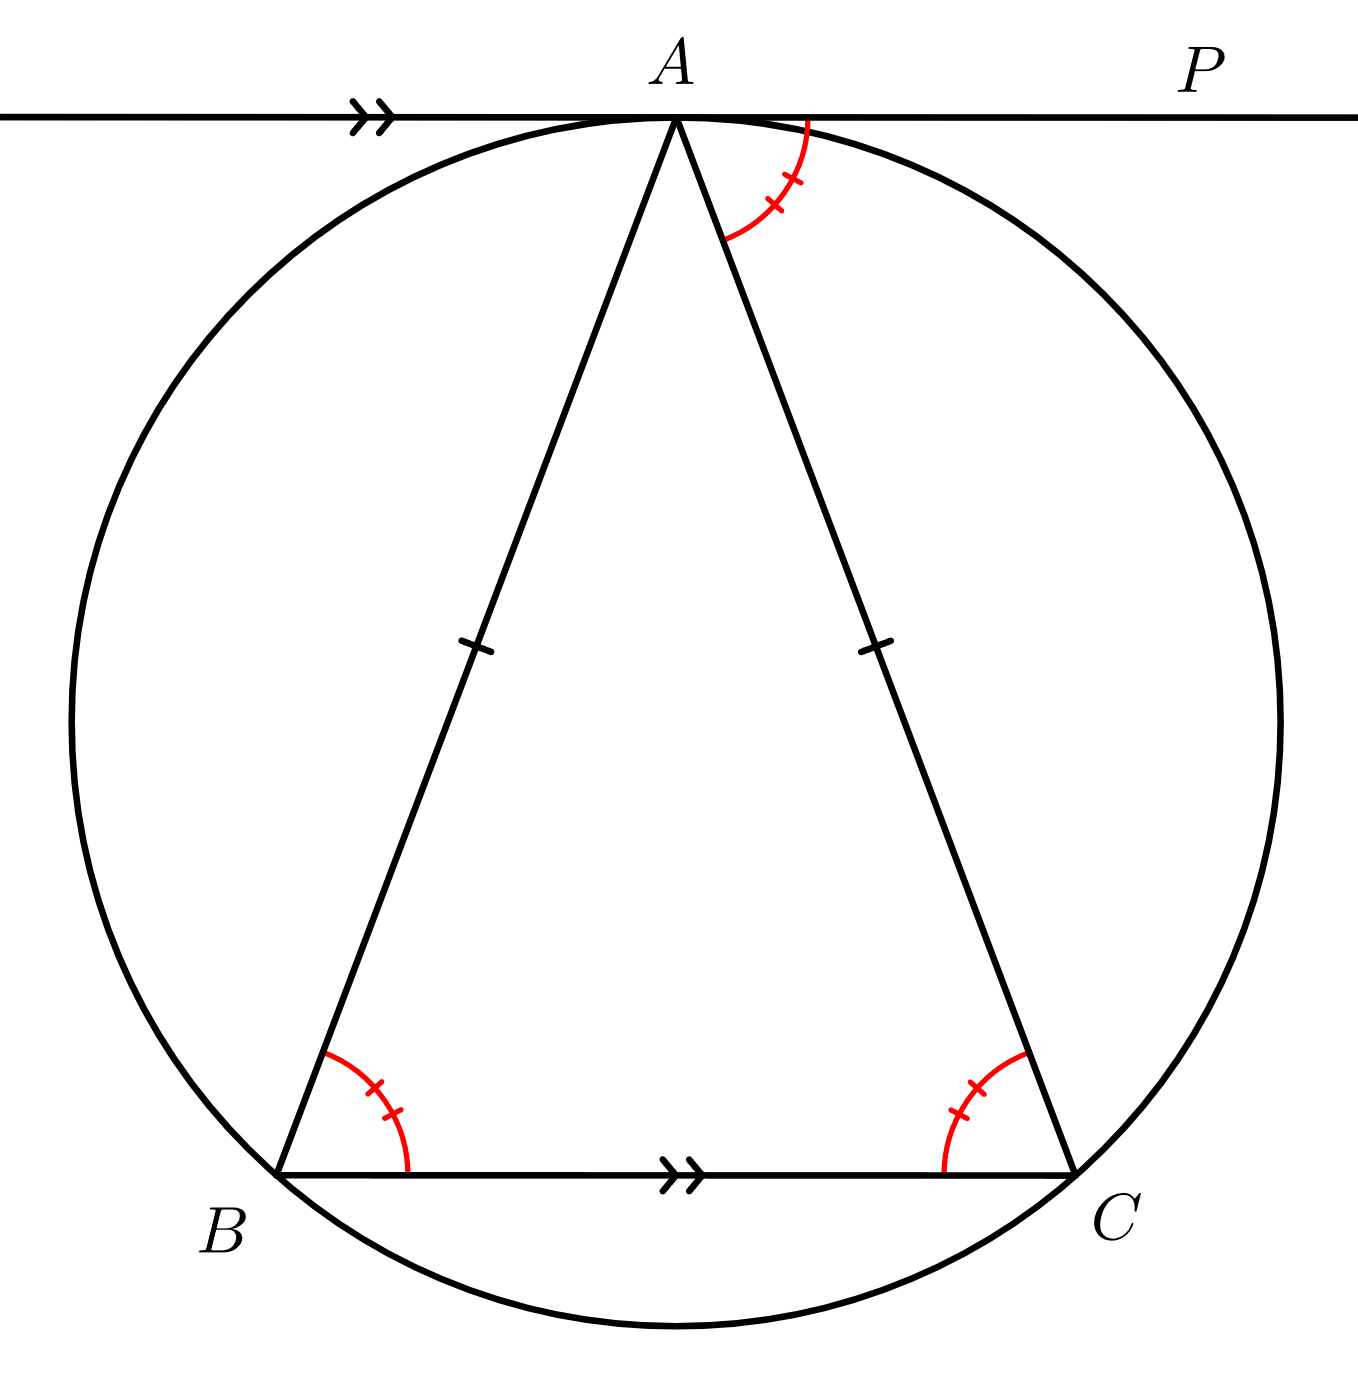
\includegraphics[width=0.6\linewidth]{images/t3i1.png}
    \end{figure}
\end{demostracion}



No solo es posible trabajar con ángulos, sino también con longitudes. En
particular, con la potencia de un punto con respecto a una circunferencia. Esto
puede ser sumamente útil en problemas donde, más que relacionar ángulos, 
busquemos relacionar longitudes de segmentos. Lo anterior, lo podemos ver en
el siguiente resultado.
\newpage

\begin{teorema}[\textbf{Punto potencia}]
    Sea $\triangle ABC$ un triángulo con circuncírculo $\Omega$, y sea
    $P$ un punto sobre la recta $AB$. Se tiene que $PC$ es tangente a 
    $\Omega$ en $C$ si y solo si $PC^2 = PB \cdot PA$.
\end{teorema}

\begin{demostracion}
    Supongamos sin pérdida de la generalidad que $A$ y $P$ se encuentran
    en lados opuestos de $BC$.

    Para empezar, si $PC$ es tangente a $\Omega$ en $C$, entonces por
    el Criterio de la tangente se tiene que $\angle PCB = \angle CAP$.
    Además, es claro que $\angle BPC = \angle CPA$. En consecuencia,
    también debe cumplirse que $\angle CBP = \angle ACP$. Así, por 
    el criterio $AAA$, $\triangle PBC \sim \triangle PCA$. En consecuencia,
    \[
        \frac{PC}{PB} = \frac{PA}{PC},
    \]
    de lo cual se sigue que $PC^2 = PB \cdot PA$.

    Ahora bien, supongamos que $PC^2 = PB \cdot PA$. Entonces se tiene que
    \[
        \frac{PC}{PB} = \frac{PA}{PC}.
    \]
    No obstante, se sabe que $\angle BPC = \angle CPA$. Así, por 
    $LAL$, se sigue que $\triangle PBC \sim \triangle PCA$. Luego,
    $\angle PCB = \angle PAC$, por lo cual del Criterio de la tangente
    se concluye que $PC$ es tangente a $\Omega$ en $C$. $\blacksquare$

    \begin{figure}[h]
        \centering
        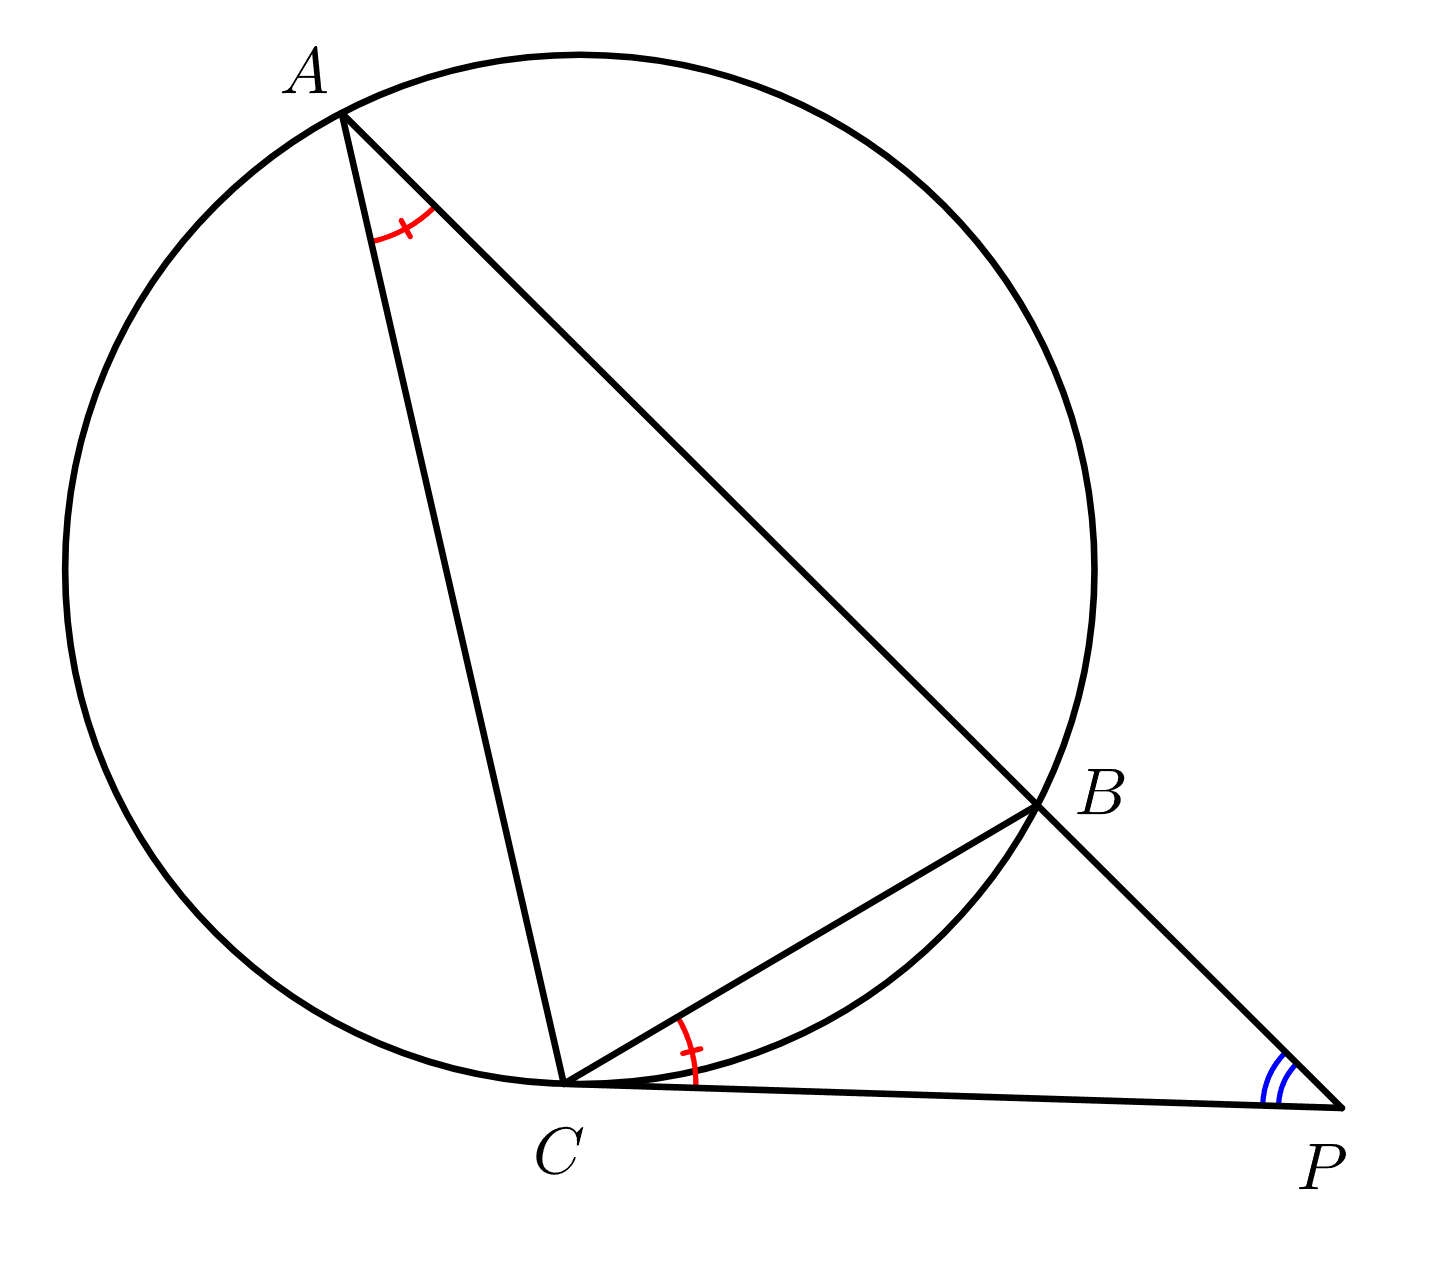
\includegraphics[width=0.6\linewidth]{images/t4i1.png}
    \end{figure}
\end{demostracion}

En la demostración del resultado anterior se usó bastante semejanza. Hay 
algunas ocasiones en que la semejanza nos interesa más que la razón 
que nos da punto potencia. Por tal razón, el siguiente teorema, en ocasiones,  
también resulta bastante útil cuando queremos trabajar con longitudes
de segmentos. En este caso, es posible deducir su demostración de lo hecho
en el teorema anterior, así que te dejaré la demostración como tarea moral
para que la pienses. No es tan complicada.

\newpage
\begin{teorema}
     Sea $\triangle ABC$ un triángulo con circuncírculo $\Omega$, y sea
    $P$ un punto sobre la recta $AB$. Se tiene que $PC$ es tangente a 
    $\Omega$ en $C$ si y sólo si $\triangle PBC \sim \triangle PCA$.
\end{teorema}

Estas no son las únicas relaciones entre segmentos que existen cuando
se tiene la tangente al circuncírculo de un triángulo. Un resultado
particularmente útil, aunque no muy conocido, relaciona dos fracciones
con las longitudes de una forma bastante inesperada.\\

\begin{teorema}
    Sea $\Omega$ una circunferencia y sean $A, B$ y $C$ puntos distintos sobre
    la misma. Además, sea $l$ la recta tangente a $\Omega$ en $A$. Sea $P$ el 
    punto de intersección de $l$ con la recta $BC$. Se tiene entonces que
    \[
        \frac{PB}{PC} = \left( \frac{AB}{AC} \right)^2.
    \]
\end{teorema}

\begin{demostracion}

    Usaremos el Teorema de la bisectriz generalizado y la Ley de senos.\\

    \begin{figure}[h]
        \centering
        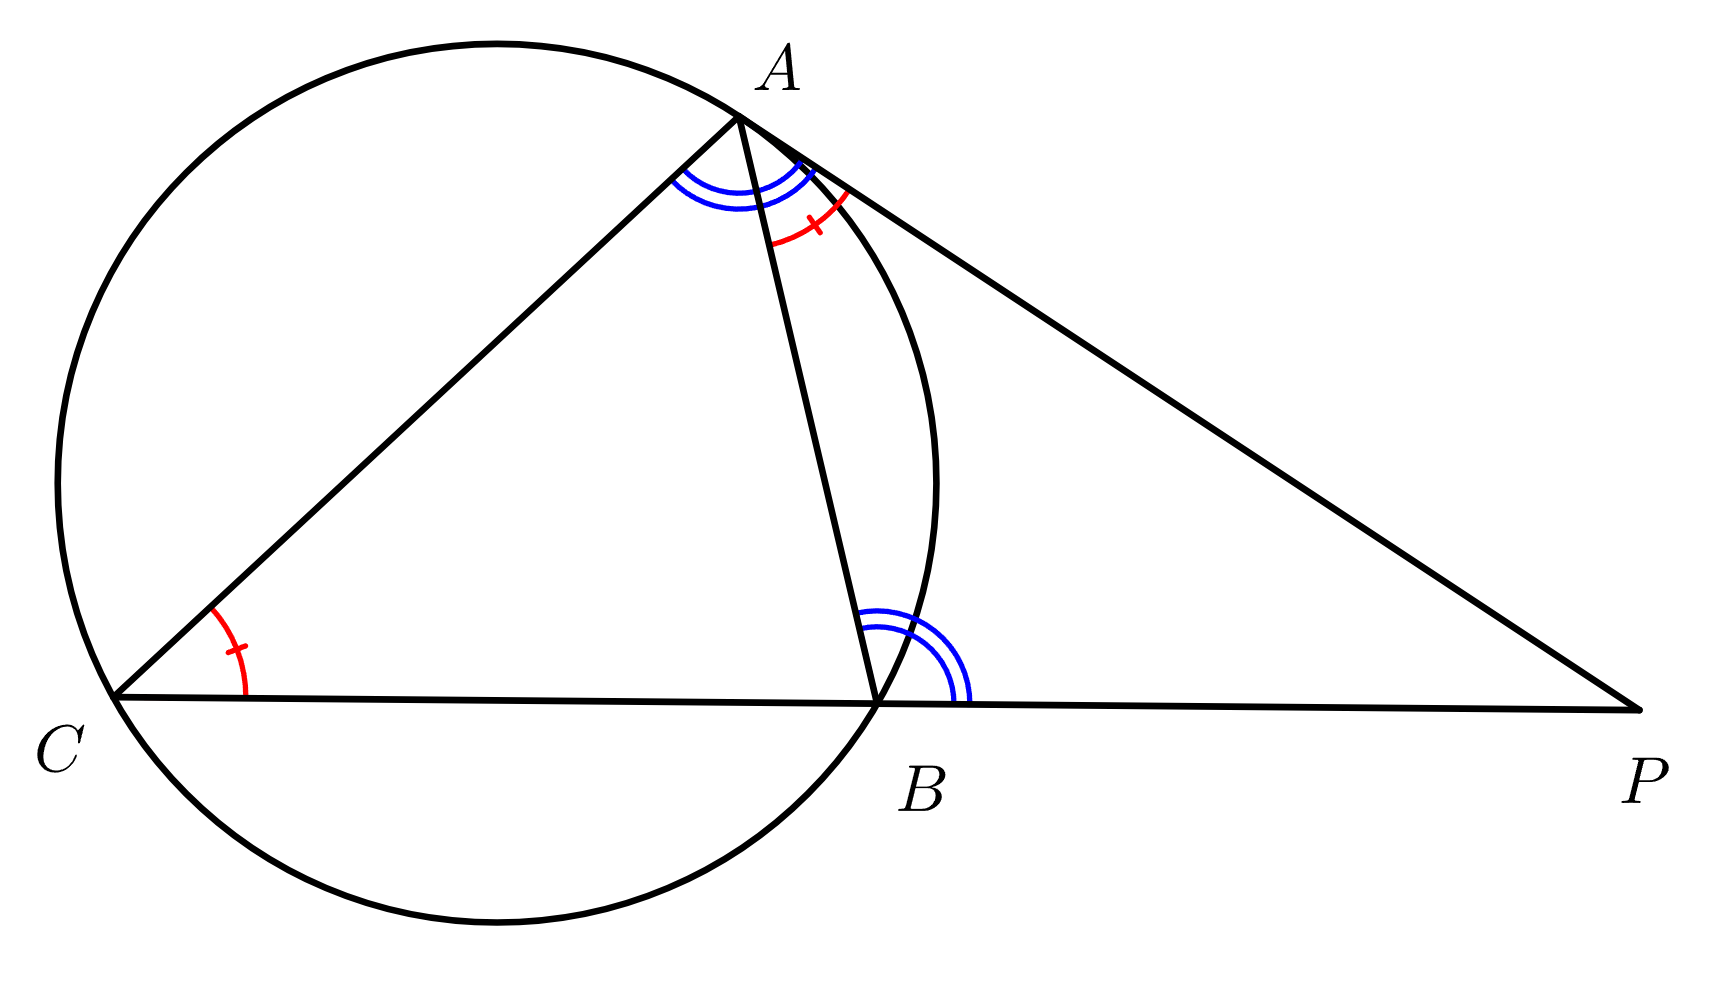
\includegraphics[width=0.8\linewidth]{images/t5i1.png}
    \end{figure}
    
    Supongamos
    sin pérdida de la generalidad que $P$  y $B$ se encuentran a lados opuestos
    de $AC$. Al ser $P$ un punto sobre la recta $BC$, entonces por el 
    Teorema de la bisectriz generalizado se cumple que
    \[
        \frac{PB}{PC} = \frac{AB}{AC}\frac{\sen \angle PAB}{\sen \angle PAC}.
    \]
    No obstante, ya que $PA$ es tangente a $\Omega$ en $A$, entonces por el
    Teorema 4, $\triangle PAC \sim \triangle PBA$, lo cual implica que
    $\angle PAB = \angle PCA = 180^{\circ} - \angle ACB$, y que
    $\angle PAC = \angle CBA$. Por tanto, 
    $\sen \angle PAB = \sen (180^{\circ} - \angle ACB) = \sen \angle ACB$ y
    $\sen \angle PAC = \sen \angle CBA$, de lo cual se deduce que
    \[
        \frac{\sen \angle PAB}{\sen \angle PAC} = 
        \frac{\sen \angle ACB}{\sen \angle CBA}.
    \]
    Asimismo, por la Ley de senos aplicada al triángulo $\triangle ABC$,
    \[
        \frac{\sen \angle ACB}{\sen \angle CBA} = \frac{AB}{AC}.
    \]
    Por lo tanto, concluimos que
    \[
        \frac{PB}{PC} = \left( \frac{AB}{AC} \right)^2. \quad \blacksquare
    \]
    
\end{demostracion}

Finalmente, quiero decir que el Criterio de la tangente, por sorprendente
que parezca, no solo sirve cuando se trata de tangencia entre círculos y 
rectas, también nos ayuda cuando se trata de circunferencias tangentes
entre sí. El teorema que sigue nos muestra un caso en el que trabajar con
circunferencias tangentes es lo mismo que trabajar con ángulos.\\

\begin{teorema}
    Sean $\triangle ABP$ y $\triangle CDP$ dos triángulos tales que 
    $ABDC$ es un cuadrilátero convexo, y tales que $P$ se encuentra dentro
    de $ABCD$. Además, sean $\omega_1$ y $\omega_2$ los circuncírculos de 
    los triángulos  $\triangle ABP$ y $\triangle CDP$, respectivamente. Se
    tiene que $\omega_1$ y $\omega_2$ son tangentes en $P$ si y sólo si
    $\angle PBA + \angle CDP  = \angle CPA$.
\end{teorema}

\begin{demostracion}
    La demostración de este teorema se basa en el hecho de que, para probar
    que dos circunferencias son tangentes en un cierto punto, basta con
    demostrar que ambas circunferencias son tangentes a alguna otra recta
    en dicho punto.\\
    
    \begin{figure}[h]
        \centering
        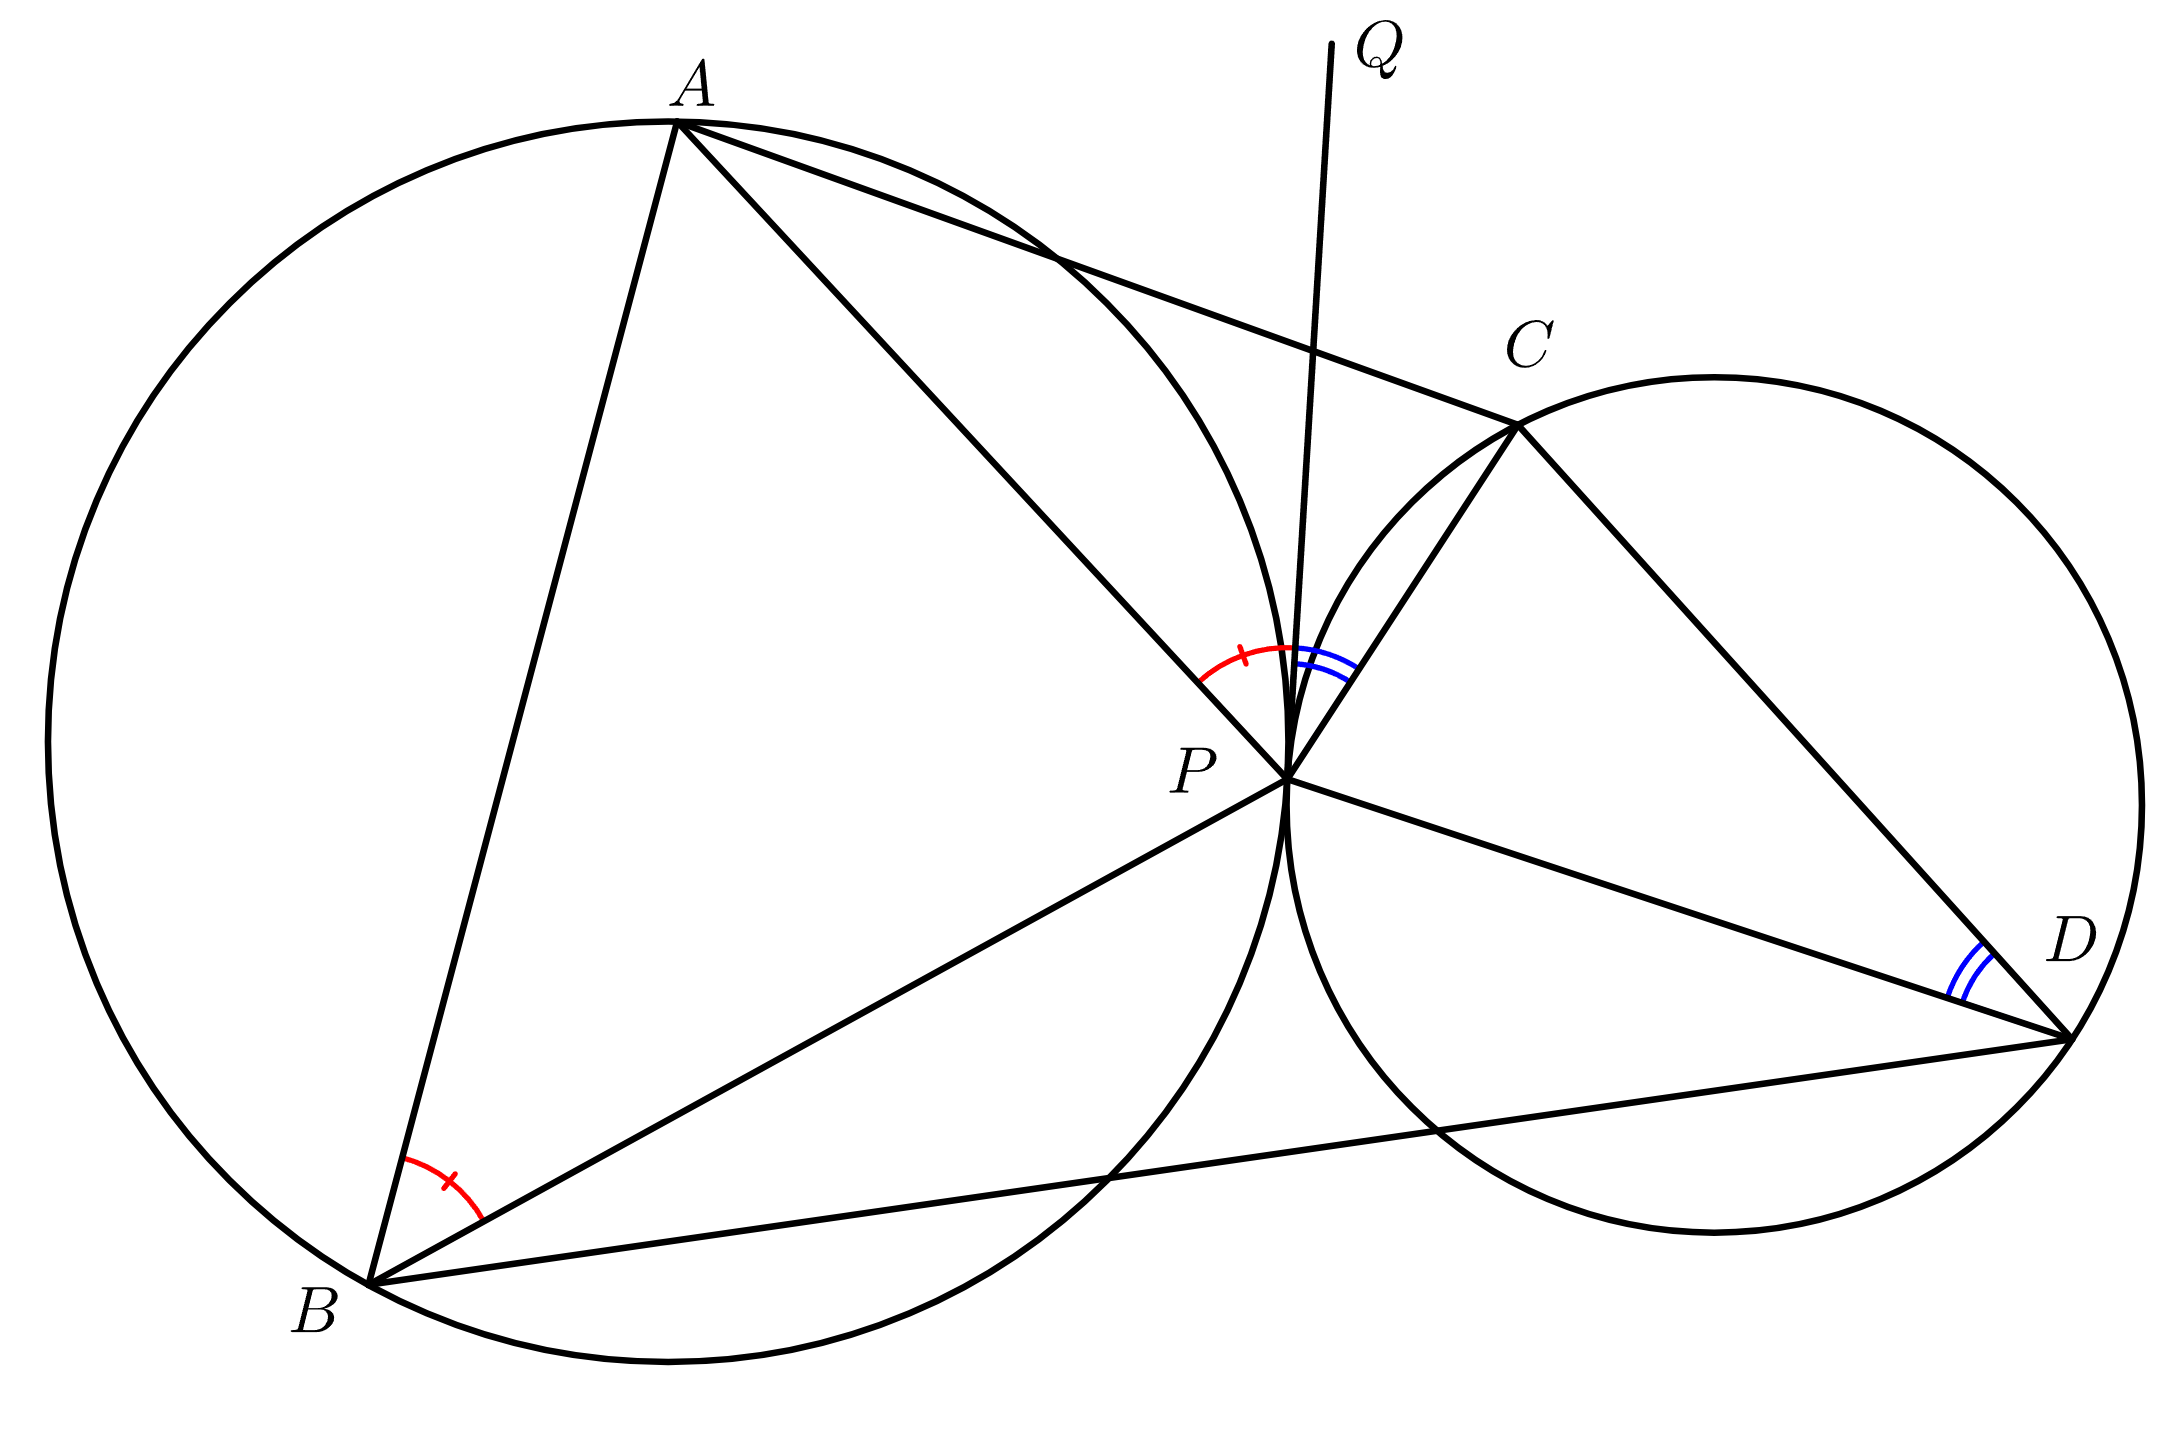
\includegraphics[width=0.8\linewidth]{images/t6i1.png}
    \end{figure}
    
    Comencemos por demostrar que si $\omega_1$ y $\omega_2$ son tangentes
    en $P$, entonces $\angle PAB + \angle CDP  = \angle CPB$. Para ello,
    sea supongamos que $\omega_1$ y $\omega_2$ son tangentes en $P$, y sea
    $l$ la recta tangente a dichas circunferencias en $P$. Además,
    sea $Q$ un punto sobre $l$ de tal manera que $Q$ y $B$ están en lados
    opuestos de $AP$. Entonces también $Q$ y $D$ están en lados opuestos
    de $CP$. Sabiendo esto, observamos que al ser $QP$ tangente
    a $\omega_1$ y a $\omega_2$ en $P$, entonces por el Criterio de la 
    tangente, $\angle QPC = \angle PBA$ y $\angle CPQ = \angle CDP$. Luego,
    ya que $\angle CPA = \angle QPA + \angle CPQ$, de lo anterior se deduce
    que $\angle CPA = \angle PBA + \angle CDP$.\\

    Por otro lado, supongamos que $\angle PBA + \angle CDP = \angle CPA$.
    En esta ocasión, sea $l$ la recta tangente al $\omega_1$ en $P$, y
    consideremos un punto $Q$ sobre $l$ tal que $Q$ y $B$ están en lados
    opuestos de $AP$. Nuevamente, $Q$ y $D$también  están en lados 
    opuestos de $CP$. Sabiendo esto, notemos que por el Criterio de la tangente,
    $\angle QPA = \angle PBA$. Luego, 
    $\angle CPQ=\angle CPA - \angle QPA = \angle CPA - \angle PBA = \angle CDP$,
    esto es, $\angle CPQ = \angle CDP$. En consecuencia, al aplicar el
    Criterio de la tangente a $\omega_2$, se obtiene que $l$ es tangente a
    $\omega_2$ en $P$. Así, al tenerse que $\omega_1$ y $\omega_2$ son tangentes
    a $l$ en $P$, concluimos que $\omega_1$ y $\omega_2$ son tangentes en $P$.
    $\blacksquare$
\end{demostracion}

\section*{Ejemplos sencillos}

Ya hemos visto muchos teoremas sobre tangentes. Ahora, ha llegado el momento
de ver algunos problemas en los que puedes usarlos. Comencemos por problemas 
relativamente sencillos.

\begin{ejemplo}
    Sea $\triangle ABC$ un triángulo con circuncentro $O$. Sea $K$ un punto
    tal que $KA$ es tangente al circuncírculo del $\triangle ABC$ y tal que
    $KC$ es perpendicular a $BC$. 
    Sea $D$ el punto de intersección de la recta $AO$ con 
    $BC$. Demuestra que $KD$ es paralela a $AB$.
\end{ejemplo}

\begin{solucion}
    Comencemos por denotar $\angle CBA = \alpha$. Como $KA$ es tangente
    al circuncírculo del $\triangle ABC$ en $A$ y $O$ es su circuncentro,
    entonces por el Criterio de la tangente, $AD$ es perpendicular a 
    $KA$. No obstante, también sabemos que $KC$ es perpendicular a $BC$. Luego,
    $ADCK$ debe ser cíclico. Aplicando nuevamente el criterio de la tangente, 
    $\angle CAK = \angle CBA = \alpha$, pero ya que $ADCK$ es cíclico, debe
    cumplirse que $\angle CDK = \angle CAK = \alpha$. Así, 
    $\angle CDK = \angle CBA = \alpha$, de lo cual se sigue que 
    $KD$ es paralela a $AB$.
\end{solucion}

\begin{ejemplo}
    Sea $ABCD$ un cuadrado (con los vértices en sentido horario) y 
    $P$ un punto en el lado $BC$ distinto de $B$ y de $C$. Considera el 
    cuadrado $APRS$ (con los vértices en el sentido horario). Demuestra 
    que la recta $CR$ es tangente a la circunferencia circunscrita del
    triángulo $ABC$.
\end{ejemplo}

\begin{solucion}
    Comencemos por un diagrama.
\end{solucion}

\begin{ejemplo}
    Sea $ABCD$ un trapecio isósceles con $AB || CD$ y donde $DC = 2AB$.
    Sean $O$ el punto de intersección de sus diagonales y $S$ la circunferencia
    con centro en $O$ que pasa por $A$ y $B$. Si $S$ es tangente a $DC$, 
    encuentra los ángulos del trapecio y demuestra que $S$ también es tangente a 
    los lados $AD$ y $BC$.
\end{ejemplo}

\begin{solucion}
    Para empezar,
\end{solucion}

Muy bien, esos fueron los ejemplos sencillitos. Sin embargo, sé que, si
estás leyendo esto, es probable que te gusten más los problemas de 
olimpiadas más avanzadas, como olimpiadas regionales, nacionales, e incluso
internacionales. Por tal razón, ahora veremos ejemplos de ese tipo de 
olimpiadas.

\section*{Ejemplos de Olimpiada}

\begin{ejemplo}[\textbf{Olimpiada Regional de México Zona Sureste, 2019}]
    Sea $ABCD$ un cuadrilátero convexo. Suponga que la circunferencia con 
    centro $B$ y radio $BC$ es tangente a $AD$ en $F$ y que la circunferencia
    con centro $A$ y radio $AD$ es tangente a $BC$ en $E$. Demuestra que $DE$
    y $CF$ son perpendiculares.
\end{ejemplo}

\begin{solucion}
    Para empezar, ya que
\end{solucion}

\begin{ejemplo}[\textbf{Olimpiada Regional de México Zona Centro, 2010}]
    En el triángulo acutángulo $\triangle ABC$, $\angle BAC$ es menor que
    $\angle ACB$. Sea $AD$ un diámetro de $\omega$, la circunferencia
    circunscrita de dicho triángulo. Sea $E$ el punto de intersección del rayo 
    $AC$ y la tangente a $\omega$ que pasa por $B$. La perpendicular a $AD$ que
    pasa por $E$ intersecta de nuevo a la circunferencia circunscrita del 
    triángulo $\triangle BCE$ en el punto $F$. Demuestra que $CD$ es bisectriz
    del $\angle BCF$.
\end{ejemplo}

\begin{solucion}
    Comencemos por demostrar que $F$ está sobre la recta $AB$. Para ello,
    sea $F'$ el punto de intersección de $AB$ con la perpendicular 
    de $E$ a $AD$, y denotemos por $\angle BCA = \alpha$ y 
    $\angle CAB = \beta$.
\end{solucion}

\begin{ejemplo}[\textbf{Olimpiada Regional de México Zona Centro, 2015}]
    En el triángulo $\triangle ABC$, tenemos que $\angle BAC$ es agudo.
    Sea $\Gamma$ el círculo que pasa por $A$ y es tangente al lado
    $BC$ en $C$. Sea $M$ el punto medio de $BC$ y sea $D$ el otro 
    punto de intersección de $\Gamma$ con $AM$. Si $BD$ corta de nuevo 
    a $\Gamma$ en $E$, demuestra que $AC$ es la bisectriz del $\angle BAE$.
 \end{ejemplo}

\begin{solucion}
    Comencemos por demostrar que $D$ está sobre la circunferencia que 
    pasa por $A$ y es tangente a $BC$ en $B$. Para ello, sea 
    $\Omega$ la circunferencia que pasa por $A$ y es tangente a $BC$ en 
    $B$. Ya que $MC$ es tangente a $\Gamma$ en $C$, entonces por punto
    potencia, $MC^2 = MD \cdot MA$. No obstante, al ser $M$ el punto 
    medio de $BC$, $MC = MB$. En consecuencia, $MB^2 = MD \cdot MA$,
    por lo que al aplicar punto potencia se obtiene que 
    $MB$ es tangente a $\Omega$ en $B$.
\end{solucion}

\begin{ejemplo}[\textbf{OMM, 2014}]
    Sea $ABCD$ un rectángulo con diagonales $AC$ y $BD$. Sean $E$ el punto de intersección de la bisectriz del ángulo $\angle CAD$ con el segmento $CD$, $F$ el punto sobre el segmento $CD$ tal que $E$ es el punto medio de $DF$ y $G$ el punto sobre la recta $BC$ tal que $BG = AC$ (con $C$ entre $B$ y $G$).
    Muestra que la circunferencia que pasa por $D, F$ y $G$ es tangente a $BG$.
\end{ejemplo}

\begin{solucion}
    Va a haber Teorema de la bisectriz normalito.
\end{solucion}

\begin{ejemplo}
    Sean $A$ y $B$ los puntos de intersección de los círculos $\omega$ y
    $\omega'$. Latangente a $\omega$ en $A$ intersecta a $\omega'$ en $C$
    y la tangente a $\omega'$ en $A$ intersecta a $\omega$ en $D$. Suponga
    que la bisectriz interior del $\angle CAD$ intersecta a $\omega$ y 
    $\omega'$ en $E$ y $F$, respectivamente, y la bisectriz externa del 
    $\angle CAD$ intersecta a $\omega$ y $\omega'$ en $X$ y $Y$, 
    respectivamente. Demuestra que la mediatriz de $XY$ es tangente al 
    circuncírculo del triángulo $\triangle BEF$.
\end{ejemplo}

\begin{solucion}
    Mucho criterio de la tangente. El punto de tangencia es la intersección
    de $XE$ con $YF$. NO USES ROTOHOMOTECIA EN ESTE PAPER.
\end{solucion}

\begin{ejemplo}[\textbf{IGO Avanzado, 2016}]
    En el cuadrilátero convexo $ABCD$, sea $P$ el punto de intersección de
    $AC$ y $BD$. Suponga que $I_1$ e $I_2$ son los incentros de los 
    triángulos $\triangle PAB$ y $\triangle PDC$, respectivamente. Sea $O$
    el circuncentro del $\triangle PAB$, y $H$ el ortocentro del 
    $\triangle PDC$. Demuestra que los circuncírculos de los triángulos 
    $\triangle AI_1B$ y $\triangle DHC$ son tangentes si y sólo si los 
    circuncírculos de los triángulos $\triangle AOB$ y $\triangle DI_2C$
    son tangentes.
\end{ejemplo}

\begin{solucion}
    Checa el solucionario de la IGO.
\end{solucion}

Las tangentes también son de mucha utilidad a la hora de trabajar con 
punto medios. Para ejemplificar esto, mostramos un último ejemplo de la 
lista corta de la IMO.\\

\begin{ejemplo}[\textbf{Lista corta de la 47 $^{\textrm{\textbf{a}}}$ IMO, 2006}]
    Sea $ABCDE$ un cuadrilátero convexo tal que
    $\angle BAC = \angle CAD = \angle DAE$ y 
    $\angle CBA = \angle DCA = \angle EDA$. Las diagonales $BD$ y $CE$ 
    se cortan en $P$. Demuestra que $AP$ biseca al lado $CD$.
\end{ejemplo}

\begin{solucion}
    Para no usar Rotohomotecia, sea $P'$ la intersección de los circuncírculos
    de los triángulos $\triangle ADE$ y $\triangle ABC$. Demuestra que 
    $P = P'$. Después usa tangentes y punto potencia.
\end{solucion}

\begin{ejemplo}[\textbf{IGO Intermedio, 2016}]
    Sea $\omega$ el ciruncírculo del triángulo rectángulo $\triangle ABC$
    ($\angle A = 90^{\circ}$). La tangente a $\omega$ en el punto $A$ intersecta
    a la recta $BC$ en el punto $P$. Suponga que $M$ es el punto medio del 
    arco menor $AB$, y $PM$ intersecta $\omega$ por segunda vez en $Q$. La 
    tangente a $\omega$ en el punto $Q$ intersecta $AC$ en $K$. Demuestra que 
    $\angle PKC = 90^{\circ}$.
\end{ejemplo}

\begin{solucion}
    Pie de la simediana externa y algunas semejanzas.
\end{solucion}

\section*{Ejercicios}

Finalmente, te dejo algunos ejercicios para que practiques tus demostraciones
con tangentes.

\begin{ejercicio}
    Sea $\triangle ABC$ un triángulo, y sean $D, E$ los pies de las 
    alturas desde $B$ y $C$, respecitvamente. Sea $M$ el punto medio de
    $BC$, y denotemos por $\Omega$ al circuncírulo del triángulo 
    $\triangle ADE$. Demuestra que $MD$ y $ME$ son tangentes a $\Omega$.
\end{ejercicio}

\begin{ejercicio}[\textbf{Olimpiada Regional de México Zona Centro, 2016}]
    Sea $A$ uno de los dos puntos donde los círculos cuyos centros son los
    puntos $M$ y $N$ se intersectan. Las tangentes en $A$ a dichos círculos
    los intersectan de nuevo en $B$ y $C$, respectivamente. Sea $P$ un punto
    tal que $AMPN$ es un paralelogramo. Demuestra que $P$ es el circuncentro
    del triángulo $\triangle ABC$.
\end{ejercicio}

\begin{ejercicio}[\textbf{Olimpiada Regional de México Zona Oeste, 2024}]
    Sea $\triangle ABC$ un triángulo y $\omega$ su circuncírculo. La tangente
    a $\omega$ que pasa por $B$ corta a la paralela a $BC$ que pasa por $A$
    en $P$. La recta $CP$ corta al circuncírulo del triángulo $\triangle ABP$
    de nuevo en $Q$, y la recta $AQ$ corta a $\omega$ en $R$. Demuestra que
    $BQCR$ es un paralelogramo si y sólo si $AC = BC$.
\end{ejercicio}

\begin{ejercicio}[\textbf{IGO Intermedio, 2016}]
    Las circunferencias $C_1$ y $C_2$ se intersectan en los puntos $A$ y 
    $B$. La tangente a $C_1$ en $A$ intersecta a $C_2$ en $P$ y la recta
    $PB$ intersecta a $C_1$ por segunda vez en $Q$ (suponga que $Q$ está
    afuera de $C_2$). La tangente a $C_2$ desde $Q$ intersecta a $C_1$ y $C_2$
    en $C$ y $D$, respectivamente (los puntos $A$ y $D$ están en lados distintos
    de la recta $PQ$). Demuestra que $AD$ es la bisectriz del $\angle CAP$.
\end{ejercicio}

\begin{ejercicio}[\textbf{Olimpiada Regional de México Zona Sureste, 2018}]
    Sean $\triangle ABC$ un triángulo isósceles con $CA = CB$ y $\Gamma$
    circuncírculo. La perpendicular a $CB$ que pasa por $B$ intersecta a 
    $\Gamma$ en los puntos $B$ y $E$. La paralela a $BC$ que pasa 
    por $A$ intersecta a $\Gamma$ en los puntos $A$ y $D$. Sean $F$ la 
    intersección de $ED$ y $BC$, $I$ la intersección de $BD$ y $EC$, 
    $\Omega$ el circuncírculo del triángulo $\triangle ADI$ y $\Phi$ 
    el circuncírulo del $\triangle BEF$. Si $O$ y $P$ son los centros de 
    $\Gamma$ y $\Phi$, respectivamente, demuestra que $OP$ es tangente a 
    $\Omega$.
\end{ejercicio}

\begin{ejercicio}[\textbf{Olimpiada Regional de México Zona Sureste, 2019}]
    Sea $\Gamma$ una circunferencia, $T$ un punto sobre $\Gamma$, y $P, A$
    dos puntos fuera de $\Gamma$ tales que $PT$ es tangente a $\Gamma$ y 
    $PA = PT$. Sea $C$ un punto sobre $\Gamma (C \neq T)$. $AC$ y $PC$
    intersectan de nuevo a $\Gamma$ en $D$ y $B$, respectivamente. $AB$
    intersecta a $\Gamma$ en $E$. Demuestra que $DE$ es paralela a $AP$.
\end{ejercicio}

\begin{ejercicio}[\textbf{IMO, 2017}]
    Sean $R$ y $S$ puntos distintos sobre el círculo $\Omega$ tales que 
    $RS$ no es un diámetro. Sea $l$ la recta tangente a $\Omega$ en $R$.
    El punto $T$ es tal que $S$ es el punto medio del segmento $RT$. El punto
    $J$ se elige en el arco menor $\widehat{RT}$ de $\Omega$ de tal manera que
    el circuncírculo $\Gamma$ del $\triangle JST$ intersecta a $l$ en 
    dos puntos distintos. Sea $A$ el punto de intersección de $\Gamma$ y $l$
    que está más cerca de $R$. La recta $AJ$ corta a $\Omega$ de nuevo en $K$.
    Demuestra que la recta $KT$ es tangente a $\Gamma$.
\end{ejercicio}

\begin{ejercicio}[\textbf{OMM, 2016}]
    Sean $ABCD$ un cuadrilátero inscrito en una circunferencia, $\ell_1$ la recta paralela a $BC$ que
    pasa por $A$ y $\ell_2$ la recta paralela a $AD$ que pasa por $B$. La recta $DC$ corta a $\ell_1$ y $\ell_2$ en los
    puntos $E$ y $F$, respectivamente. La recta perpendicular a $\ell_1$ que pasa por $A$ corta a $BC$ en
    $P$ y la recta perpendicular a $\ell_2$ por $B$ corta a $AD$ en $Q$. Sean $\Gamma_2$ y $\Gamma_1$ las circunferencias
    que pasan por los vértices de los triángulos $ADE$ y $BFC$, respectivamente. Demuestra
    que $\Gamma_1$ y $\Gamma_2$ son tangentes si y sólo si $DP$ es perpendicular a $CQ$.
\end{ejercicio}

\begin{ejercicio}[\textbf{EGMO, 2015}]
    Sea $\triangle ABC$ un triángulo acutángulo, y sea $D$ el pie de la 
    altura desde $C$. La bisectriz del $\angle ABC$ intersecta $CD$ en 
    $E$ y corta al circuncírculo $\omega$ del triángulo $\triangle ADE$
    de nuevo en $F$. Si $\angle ADF = 45^{\circ}$, demuestra que $CF$ es 
    tangente a $\omega$.
\end{ejercicio}

\end{document}